\documentclass[a4paper, 12pt]{report}

\usepackage{pdfpages}
\usepackage[ra={Livrable 1 - P2I2}, subjectAcronym=PPII2]{configfrancaisCM}

\title{Rapport}
\author{DIONISIO, FREY, BILLARD, MEZUREUX}
\date{\today}

\begin{document}

\maketitle
\dominitoc
\mtcsettitle{minitoc}{}
\tableofcontents

\chapter{Introduction}
\minitoc
\chaptermark{Introduction}
\clearpage

\section{Contexte et objectifs du projet}

Ce projet s'inscrit dans le cadre pédagogique de notre première année d'étude en école d'ingénieur au sein de l'établissement TELECOM Nancy. L'objectif y est de mettre en pratique les compétences scientifiques et techniques acquises tout au long de cette première année en se rapprochant d'une étude de cas concrète.
\bigskip

Il se divise en deux étapes distinctes. Il nous a été demandé dans un premier temps de construire en langage "C" un programme qui permet de planifier un parcours de charge pour un véhicule électrique et pour un trajet donné et d'enrichir cette application en y incorporant les ajouts de notre choix. Dans un second temps, il nous a fallu réaliser, toujours en langage "C", un module de simulation qui pour un ensemble d'usagers, calcule le taux de charge des bornes du territoire.
\bigskip

Notons également que tout au long du projet nous avons dû suivre une gestion de projets rigoureuse, ce
qui nous a permis d’assurer une planification efficace et un suivi approprié des activités. Nous étions
obligé d'adopter une approche méthodologique solide, afin d’assurer que notre projet soit réalisé de manière efficace, dans les délais impartis.
\bigskip

Toute l’équipe a pris plaisir à travailler sur le projet et nous tenons à remercier tous ceux qui nous
ont aidés.

\section{Objectifs du rapport}

Ce rapport synthétise le travail réalisé par l'équipe de PoinCarWash pour répondre à la problématique posée. À savoir travailler à l'élaboration d'outils utiles au développement d'une mobilité plus écologique.

\bigskip
Le présent rapport fait état de la conception et de l'implémentation de notre travail mais également des performances et des tests sur ce dernier, ainsi que d'une présentation de notre gestion de projet.

\section{Présentation du plan}

Au cours de ce rapport, nous aborderons dans un premier temps les éléments de gestion de projet communs aux deux étapes. Cette première partie nous permettra ainsi de justifier nos choix d'approches méthodologiques pour la réalisation de ce projet.
\bigskip

Nous procéderons ensuite de manière similaire pour les deux étapes du projet. En premier lieu, nous décrirons les éléments de gestion de projet spécifiques à chacune d'entre elles. Nous détaillerons ensuite les phases de conception et de développement avant d'enfin présenter les performances et les tests de nos applications.
\bigskip


Pour conclure nous récapitulerons les résultats obtenus dans chaque partie du projet en les mettant en parallèle avec les objectifs fixés au départ, nous analyserons les avantages et les limites de notre travail, et formulerons des recommandations pour de futures améliorations et développements avant de conclure définitivement le projet.


\chapter{Gestion de projet}
\minitoc
\chaptermark{Gestion de projet}
\clearpage
\section{Définition du projet}

\subsection{Contexte et justification du projet}

Avec la prise de conscience écologique grandissante dans la population, les citoyens et les Etats se tournent progressivement vers des modes de consommation et des politiques plus responsables et écologiques. La Commission européenne a dans cette optique récemment pris la décision d'interdire la vente de véhicules thermiques à l'horizon 2035. Le développement et l'utilisation des véhicules électriques va donc connaître une croissance élevée dans les années à venir. En effet, selon les premières projections\footnotemark[1], le marché des véhicules électirifiés pourrait représenter 24\% des parts de marché d'ici 2025 et 90\% d'ici 2040.
\bigskip
\footnotetext[1]{Selon l'étude \href{https://about.bnef.com/electric-vehicle-outlook/}{BloombergNEF}}

Pourtant, voyager dans ce type de véhicules peut encore parfois s'avérer difficile, notamment en ce qui concerne leur autonomie toujours relativement limitée et la répartition des bornes de recharge sur le territoire, cette dernière étant encore très inégale sur le sol français. Il est donc nécessaire pour faciliter leur adoption d'en faciliter et d'en optimiser l'utilisation.
\bigskip

La première étape de notre projet consiste alors en la conception d'un algorithme permettant de calculer pour un utilisateur le trajet le plus court entre deux endroits situés en France, en optimisant ses passages aux bornes de recharges. Cet outil pourra aider les conducteurs à naviguer plus efficacement et à ainsi surmonter les inquiétudes liées à l'autonomie limitée des voitures électriques.
\bigskip

La seconde étape du projet est basée sur l'étude du remplissage des stations en fonction d'un ensemble de trajets donnés. L'acquisition de ces statistiques pourrait par exemple permettre de planifier plus efficacement l'expansion future du réseau de recharge.
\bigskip

Ainsi nous espérons au travers de ce projet promouvoir une mobilité plus durable en participant à l'élaboration de solutions pratiques pour surmonter les obstacles liés à l'autonomie et à la disponibilité de stations de recharge pour véhicules électriques.
\bigskip

\subsection{Portée du projet}

\textbf{\underline{Objectifs du projet} :}
\begin{itemize}
    \item Conception d'un algorithme de calcul d'itinéraire optimisé pour véhicule électrique
    \item Conception d'une application d'analyse du remplissage des stations de recharge
\end{itemize}
\bigskip

\textbf{\underline{Ressources} :}
\begin{itemize}
    \item Groupe de projet (4 personnes) : temps de travail variable pendant 9 semaines
    \item Equipe pédagogique de TELECOM Nancy : aide ponctuelle
    \item Bases de données relatives aux stations de recharge et aux véhicules électriques
\end{itemize}
\clearpage

\textbf{\underline{Livrables} :}
\begin{itemize}
    \item Code source des deux applications, \textbf{24 Mai}
    \item Guide utilisateur décrivant l'installation du programme et les modalités de son utilisation, \textbf{24 Mai}
    \item Rapport du projet incluant les éléments relatifs à la gestion de projet et décrivant les choix motivés des structures de données et des algorithmes (sur la base d'un état de l'art détaillé), les
          fonctions réalisées et leur analyse (complexité mémoire, temps), les fonctions réalisées et les tests mis en œuvre, \textbf{24 Mai}
\end{itemize}
\bigskip

\textbf{\underline{Éléments non prévus dans le projet} :}
\begin{itemize}
    \item Adaptation du calcul des itinéraires en fonction du taux de remplissage des stations de recharges.
\end{itemize}

\subsection{Parties prenantes}

\textbf{\underline{Identification} :}
\begin{itemize}
    \item Interne :
          \begin{itemize}
              \item Groupe de projet : Les participants directs au projet, responsables de la conception et du développement des outils demandés.
          \end{itemize}
    \item Externe :
          \begin{itemize}
              \item Enseignants et jury : Ils guident et évaluent les étudiants dans le cadre du projet.
              \item Autres groupes : D'autres groupes de projet travaillant sur des sujets similaires, avec lesquels des échanges et des discussions peuvent être initié pour partager des idées et des connaissances.
          \end{itemize}
\end{itemize}
\bigskip

\textbf{\underline{Evaluation de l'influence et de l'importance} :}
\begin{itemize}
    \item Groupe de projet : Influence élevée et importance élevée, car ils sont directement responsables de la réalisation du projet et de l'atteinte des objectifs fixés.
    \item Enseignants/jury : Influence élevée et importance élevée, car ils évalueront le projet et fourniront des conseils et des orientations pour assurer la qualité et la réussite du projet.
    \item Autres groupes de projet : Influence faible à moyenne et importance faible à moyenne, car ils peuvent partager des connaissances et des expériences similaires, mais leur impact direct sur le projet est limité.
\end{itemize}
\bigskip

On peut synthétiser cette analyse au travers de ce diagramme:

\begin{center}
    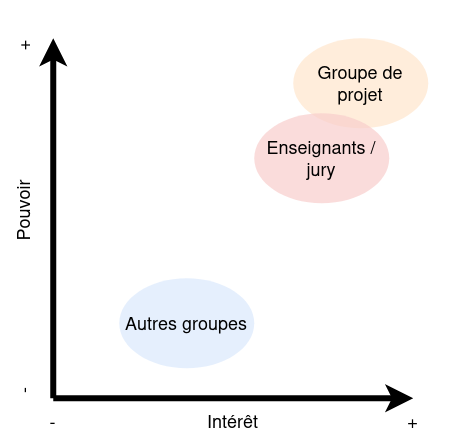
\includegraphics[width = 0.45\textwidth]{IMG/parties_prenantes.png}
\end{center}

\textbf{\underline{Plan d'action} :}
\begin{itemize}
    \item Groupe de projet :
          \begin{itemize}
              \item Communiquer de façon régulière et transparente au sein du groupe.
              \item Organiser des réunions pour discuter des progrès réalisés, des difficultés rencontrées et des décisions à prendre.
          \end{itemize}
    \item Enseignants/jury :
          \begin{itemize}
              \item Communiquer de façon ponctuelle pour s'assurer que nous travaillons toujours dans la bonne direction.
              \item Solliciter leur aide en cas de trop grosse difficulté.
          \end{itemize}
    \item Autres groupes de projet :
          \begin{itemize}
              \item Echanger de façon ponctuelle pour recueillir des idées, des connaissances ou des expèriences supplémentaires.
          \end{itemize}
\end{itemize}

\subsection{Contraintes et risques}

\textbf{\underline{Contraintes} :}
\begin{itemize}
    \item Temporelle :
          \begin{itemize}
              \item Le projet doit être réalisé en 9 semaines.
          \end{itemize}
    \item Techniques :
          \begin{itemize}
              \item Langage de programmation : le langage utilisé doit être le langage "C".
          \end{itemize}
\end{itemize}
\bigskip

\textbf{\underline{Risques} :}
\begin{itemize}
    \item Techniques :
          \begin{itemize}
              \item Incompatibilités matérielles : nous ne travaillons pas tous sous le même OS.
              \item Problèmes de performance : les outils demandés peuvent demander des traitements lourds, nos machines pourraient être dépassées.
          \end{itemize}
    \item Gestion de projet :
          \begin{itemize}
              \item Gestion du temps et planification : nous ne travaillons pas à temps plein sur le projet et nos autres activités peuvent nous empêcher de consacrer suffisament de temps au projet.
          \end{itemize}
    \item Liés aux données :
          \begin{itemize}
              \item Les données utilisées pour le projet peuvent être incomplètes, inexactes ou indisponibles.
          \end{itemize}
\end{itemize}
\bigskip

\textbf{\underline{Evaluation} :}
\begin{itemize}
    \item Contrainte temporelle :
          \begin{itemize}
              \item Impact : le temps disponible pour la conception, le développement et les tests est limité.
              \item Gravité : élevée, un manque de temps peut affecter la qualité globale du projet.
          \end{itemize}
    \item Contrainte technique :
          \begin{itemize}
              \item Impact : le langage "C" est maîtrisé par l'équipe, la contrainte n'a donc que peu d'impact.
              \item Gravité : Négligeable, cette contraintes peut être gérée en planifiant un temps de formation mais cela demande du temps.
          \end{itemize}
          \clearpage % --- Pour la mise en page -> à supprimer si le contenu précédent est modifié et que la mise en page change ---

    \item Risques techniques :
          \begin{itemize}
              \item Impact : les incompatibilités matérielles peuvent entraîner des problèmes d'intégration et de compatibilité lors de la mise en œuvre. Les problèmes de performance peuvent affecter la réactivité de l'application et la satisfaction de l'utilisateur.
              \item Gravité : Modérée, ces risques peuvent être atténués en identifiant les incompatibilités dès le début du projet et en optimisant le code pour améliorer les performances.
          \end{itemize}
    \item Risque de gestion de projet :
          \begin{itemize}
              \item Impact : Une mauvaise gestion du temps et de la planification peut entraîner des retards dans l'achèvement des tâches et la réalisation à terme des objectifs du projet.
              \item Gravité : Modérée, une bonne communication et une planification efficace peuvent minimiser les impacts de ce risque.
          \end{itemize}
    \item Risque lié aux données :
          \begin{itemize}
              \item Impact : Des difficultés pour obtenir les données peuvent allonger le temps nécessaire à l'élaboration des applications, de plus des données de mauvaise qualité peuvent affecter la précision et la validité des résultats obtenus.
              \item Gravité : Modérée, des efforts de collecte et de validation des données seront nécessaires pour minimiser l'impact de ce risque.
          \end{itemize}
\end{itemize}
\bigskip

On peut synthétiser les résultats de cette analyse dans une matrice des risques :

\begin{center}
    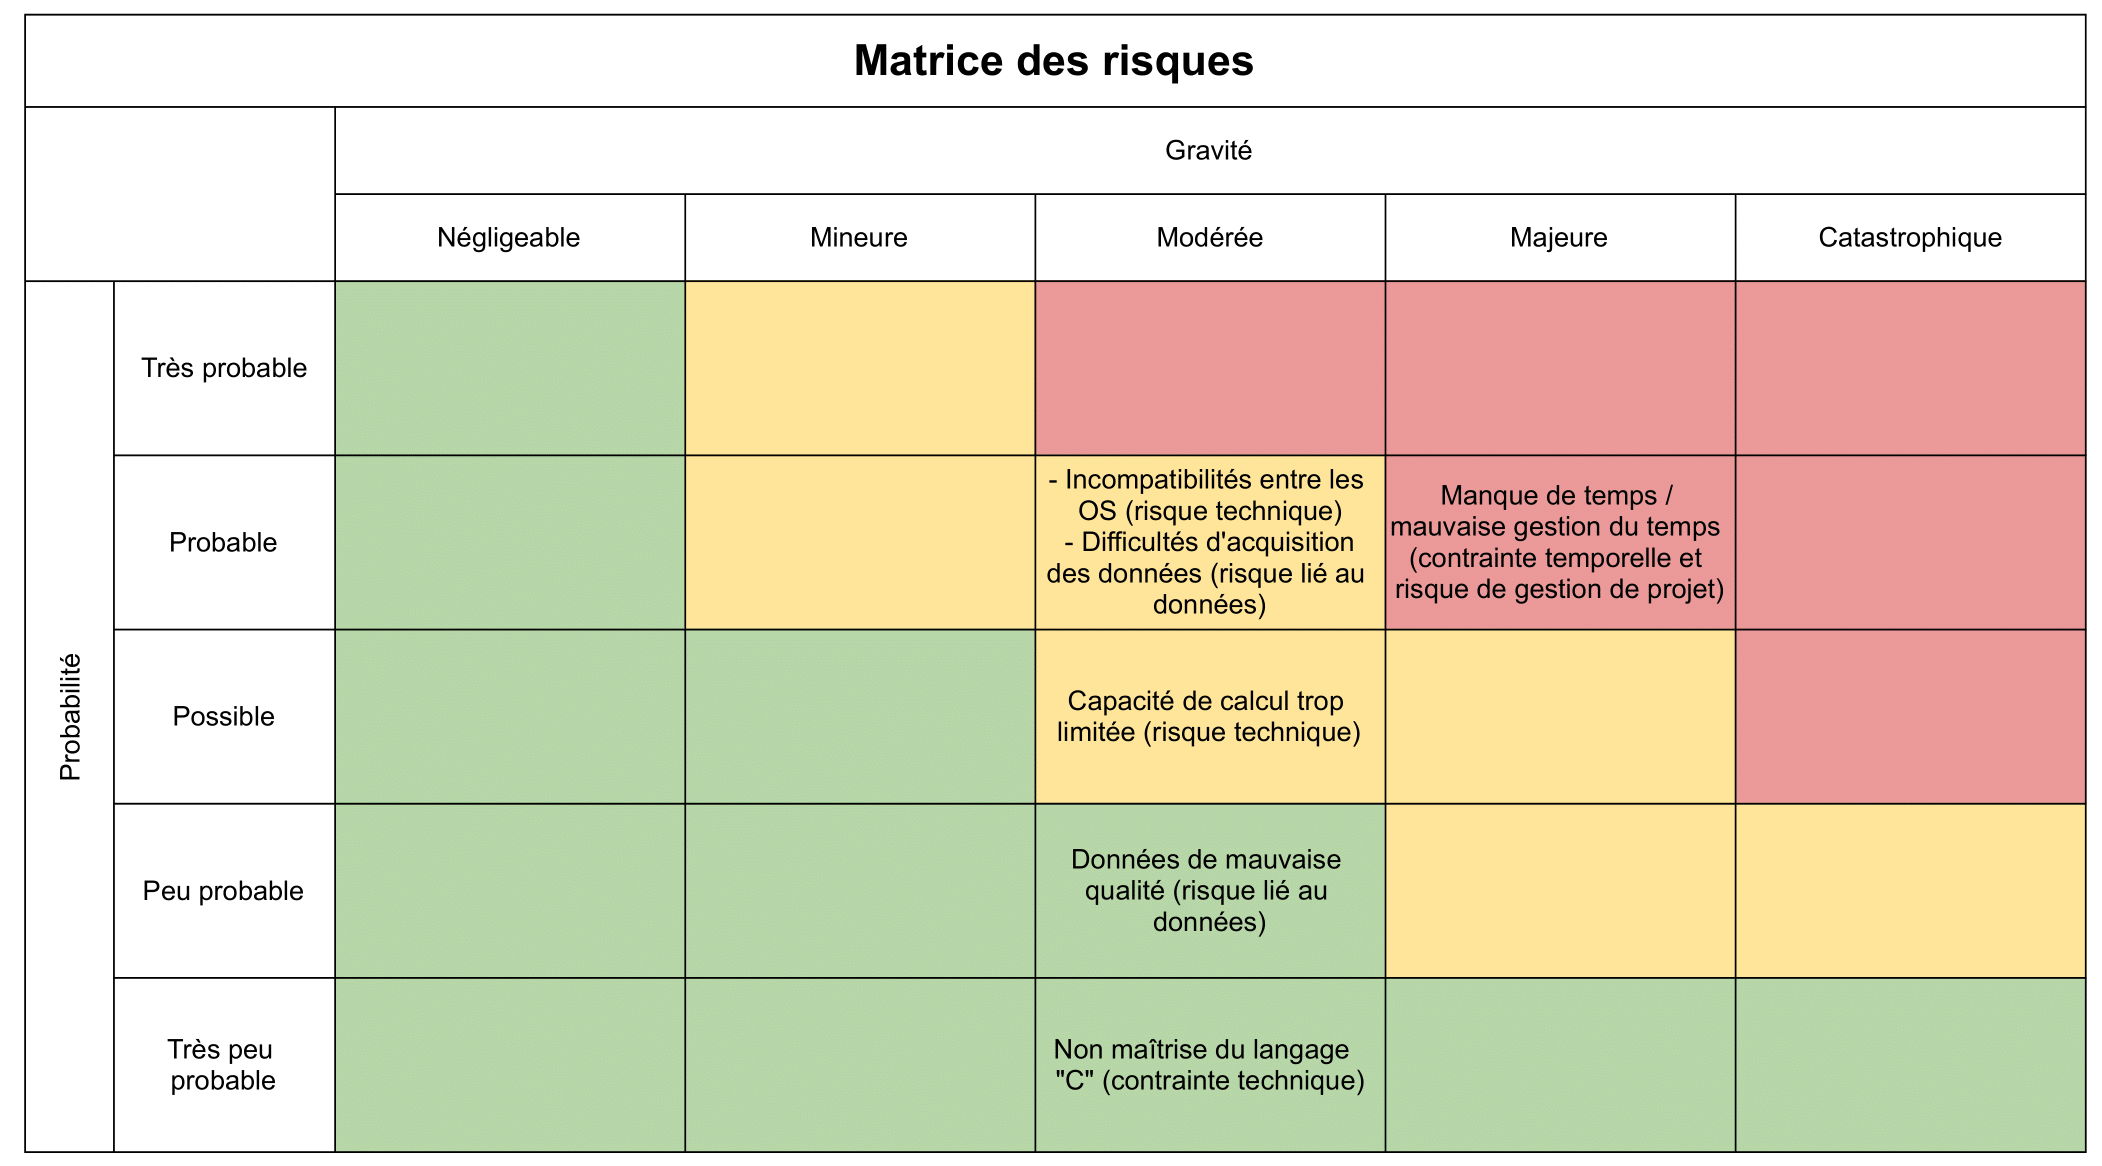
\includegraphics[width = \textwidth]{IMG/mat_risques.png}
\end{center}
\clearpage

\section{Approche et méthodologie de gestion de projet}

\subsection{Méthode de gestion de projet}

Pour ce projet nous avons décidé de nous orienter vers une gestion de projet classique pour les raisons suivantes :
\bigskip

\begin{itemize}
    \item \textbf{La précision des spécifications} : le sujet étant clair à ce niveau, nous savions dès le départ tout ce qui était attendu de nous. Ainsi, comme les livrables ne risquaient pas de changer en cours de route et que la participation des parties prenantes était limitée, une gestion agile n'était pas de mise.
          \bigskip

    \item \textbf{La structuration claire et la gestion du temps} : La gestion de projet classique offre une structure claire et bien définie avec des étapes séquentielles. Cela permet de diviser le projet en phases distinctes, ce qui facilite la planification, l'organisation et le suivi des progrès. La gestion de la contrainte temporelle en est également plus aisé.
          \bigskip

          Nous avons décidé de découper le projet ainsi :
          \begin{itemize}
              \item Semaine 1 : définition, planification et répartition du projet.
              \item Semaine 2 à 5 : conception, développement, tests et vérifications de la première étape.
              \item Semaine 5 à 8 : conception, développement, tests et vérifications de la seconde étape.
              \item Semaine 9 : Evaluation, rédaction du rapport et clôture du projet
          \end{itemize}
          \bigskip

    \item \textbf{La documentation} : La méthode classique encourage la documentation régulière des résultats intermédiaires du projet, cela renforce le suivi des activités, la détection des erreurs et simplifie l'étape de rédaction du rapport.
\end{itemize}

\subsection{Forces et faiblesses}

Pour travailler efficacement il est important de connaître les forces sur lesquelles ont peut s'appuyer, ainsi que les faiblesses auxquelles il faut faire attention.
\bigskip

\textbf{\underline{Nos forces} :}
\begin{itemize}
    \item On a de l’expérience ensemble, on a déjà eu l'opportunité de travailler de concert. On connait donc les méthodes de travail de chacun et on peut alors mieux adapter la planification, la répartition et l'organisation du travail en fonction de chaque individu. On peut également noter que l'équipe fait preuve d'une forte cohésion.
    \item Chaque membre du groupe est doté de bonnes capacités de communication. Cela sera un avantage lors de nos réunions pour se comprendre rapidement mais aussi lors de la soutenance pour  communiquer avec le jury.
    \item Notre expérience dans le domaine associatif nous a solidement formé dans les domaines relatifs à l'organisation. Ces points forts seront utiles dans tout ce qui est relatif à la gestion de projet.
\end{itemize}
\bigskip

\textbf{\underline{Nos faiblesses} :}
\begin{itemize}
    \item Nos connaissances en langage "C" sont encore très récentes, ainsi on aura de manière certaine besoin de plus temps pour développer ce type d'outils que des développeurs expérimentés.
    \item On est tous très engagés dans le mileu associatif de TELECOM et les cours nous prennent beaucoup de temps, on a donc peu de temps à consacrer au projet.  Il faudra être discipliner sur le temps que l'on arrive à dégager.
\end{itemize}
\clearpage

On peut synthétiser cette analyse sous forme de tableau :

\begin{table}[htbp]
    \centering\begin{tabular}{|c|c|}
        \hline
        \textcolor{mainColor}{Forces}                             & \textcolor{mainColor}{Faiblesses}       \\
        \hline\hline
        Forte expérience en équipe                                & Novices en langage "C"                  \\
        \hline
        Bonne capacité de communication                           & Très pris par l'associatif et les cours \\
        \hline
        Expérience solide en organisation et en gestion de projet &                                         \\
        \hline
    \end{tabular}
\end{table}

\subsection{Communication et collaboration}

\begin{itemize}
    \item \textbf{La communication interne} : Pour notre communication interne, nous avons décidé de continuer à utiliser Discord.
    \item \textbf{Les réunions} : En ce qui concerne les réunions nous avons décider dans la mesure de possible de faire une réunion d'avancement par semaine et des réunions techniques ponctuelles pour échanger sur les détails techniques. Toutes les réunions feront l'objet de compte rendu de réunion.
    \item \textbf{La répartition du travail} : Pour gérer nos ToDo, nous avons décidé d'utiliser le logiciel Trello.
    \item \textbf{Partage des ressources} : En ce qui concerne le partage des ressources et de nos avancées, nous utileserons le serveur GitLab de l'école.
\end{itemize}


\clearpage
\section{Suivi et évaluation du projet}
\subsection{Méthodes de suivi}
\subsection{Évaluation des résultats}
\subsection{Gestion des modifications}
\subsection{Évaluation de la performance}


\chapter{Première étape}
\minitoc
\chaptermark{Première étape}
\clearpage
\section{Analyse}

La première consiste à construire en langage "C" un programme qui permet de proposer à tout usager souhaitant se rendre d'un point A à un point B du territoire, un parcours de charge de son véhicule électrique.

\subsection{Etat de l'art}
\subsubsection{Le problème}
Le problème qui nous a été donné est un problème de recherche de plus court chemin. Il est alors fortement probable que nous soyons amenés à utiliser une structure de type graphe. Le problème du plus court chemin entre un sommet A et un sommet B revient à chercher le chemin de A à B où la somme des poids des arcs qu’il traverse est minimale\footnote{Si on ajoute des contraintes à ce problème comme des fenêtres de temps, le problème peut devenir NP-difficile.}. Il faut donc choisir un algorithme qui trouve des solutions à ce problème.

\subsubsection{Algorithme}
Les potentiels algorithmes pour ce problème sont :
\begin{itemize}
    \item Dijkstra
    \item A*\footnote{Cet algorithme semble le plus efficace d’après les recherches.}
    \item Bellman-Ford
    \item Viterbi
    \item Floyd-Warshall\footnotemark[3]
    \item Johnson\footnotemark[3]
\end{itemize}

\footnotetext[3]{Si l’on veut tous les chemins à partir d’un point}

\subsubsection{Applications existantes}
Ce problème ayant déjà été étudié, il existe des applications permettant de répondre aux besoins de notre sujet, notamment :

\begin{itemize}
    \item \textbf{\underline{Chargermap} :} Son fonctionnement est très simple. Il faut d’abord lancer l’application sur son smartphone Android ou Apple, puis renseigner ses points de départ et d’arrivée. Vous devez ensuite préciser le modèle de votre véhicule, les niveaux de batterie souhaités au départ comme à l’arrivée et enfin, la vitesse maximale que vous prévoyez au cours du trajet. À partir de ces informations, l’algorithme calcule en une poignée de secondes le chemin le plus adapté. L’itinéraire à suivre et les bornes où s’arrêter sont ainsi affichés sur une carte. Une feuille de route vous indique également la distance à parcourir entre chaque escale et la durée de chaque recharge. Vous verrez qu’il n’est pas systématiquement nécessaire de faire un plein complet, un appoint de quelques dizaines de minutes suffisant la plupart du temps.
    \bigskip
    \item \textbf{\underline{A Better Routeplanner} :} Le fonctionnement de cet outil est globalement similaire celui de Chargermap. Lieu de départ et d’arrivée, niveaux de batterie, modèle de véhicule : on y renseigne les mêmes informations. A Better Routeplanner (ABRP) se démarque cependant en proposant un mode expert, qui ouvre accès à un panneau extrêmement complet de données à préciser : poids des bagages et passagers, météo, consommation moyenne personnalisée, type de chargeurs, etc. Contrairement à Chargemap, ABRP présente aussi l’avantage d’estimer les prix des recharges sur sa feuille de route. Les différences de temps de charge et de parcours entre Chargemap et A Better Routeplanner sont souvent le résultat d’estimations différentes de ses concepteurs. Le premier outil peut, par exemple, être plus ou moins optimiste sur la capacité d’un véhicule à recharger rapidement que le second.
\end{itemize}

\subsection{Charte de projet}

\subsection{Planification}
\clearpage

\section{Conception}
\subsection{Manipulation des données}
L'énoncé fournit deux ressources. La première est une basse de données du gouvernement répertoriant les stations de recharges pour véhicules électriques du territoire français ainsi que diverses informations sur ces stations (nombre de bornes, puissance, \dots). La seconde est une base de données tirée du site \url{https://ev-database.org/} qui contient une kyrielle de données sur les véhicules électriques du marché (autonomie, vitesse de recharge, \dots).\par\bigskip
La première étape de cette partie consiste à extraire les données mises à notre disposition de manière à pouvoir être exploitées facilement en \texttt{C} par la suite. Pour les stations de recharge, le site du gouvernement (\href{https://www.data.gouv.fr/fr/datasets/fichier-consolide-des-bornes-de-recharge-pour-vehicules-electriques/}{serveur Etalab}) propose nativement un export au format \texttt{CSV} qui est un format qui nous  être le plus simple pour arriver à nos fins. Cependant, le site qui fournit les données sur les véhicules, lui, ne propose aucune option d'export. Nous avons donc commencé par écrire un script de \textit{parsing} en \texttt{Python} qui va récupérer les données sur le site et les enregistrer dans un fichier \texttt{CSV}. Nous n'avons récupéré que les données qui nous semblaient utiles parmis toutes celles proposées sur le site internet. C'est-à-dire le nom du véhicule, son autonomie ainsi que sa vitesse de recharge\par\bigskip
\begin{longlisting}
    \caption{Script de récupération des données sur les véhicules électriques}
    \begin{minted}[linenos]{python}
import requests
from bs4 import BeautifulSoup
import json

url = """https://ev-database.org/#sort:path~type~order=.erange_real~number~desc|
    range-slider-range:prev~next=0~1200|range-slider-acceleration:prev~next=2~23|
    range-slider-topspeed:prev~next=110~350|range-slider-battery:prev~next=10~200|
    range-slider-towweight:prev~next=0~2500|range-slider-fastcharge:prev~next=0~1500|
    paging:currentPage=0|paging:number=all"""

response = requests.get(url)
assert (response.ok)

soup = BeautifulSoup(response.text, 'html.parser')

vehicle_info = []
vehicles = soup.find_all('div', class_='list-item')[1:]  # skip header row
for vehicle in vehicles:
    vehicle_tmp = {}
    vehicle_tmp['name'] = vehicle.find('h2').text
    specs = vehicle.find('div', class_='specs').find_all('p')
    vehicle_tmp['range'] = specs[2].find_all('span')[1].text[:-3]
    vehicle_tmp['fast_charge'] = specs[4].find_all('span')[2].text

    vehicle_info.append(vehicle_tmp)

with open('vehicle_info.json', 'w') as f:
    json.dump(vehicle_info, f, indent=4)
        \end{minted}
\end{longlisting}
\subsection{Théorie des graphes}
Le problème posé dans cette première partie nous a tout de suite fait penser à la théorie des graphes et plus particulièrement à un calcul de plus court chemin. L'algorithme de \textsc{Dijkstra}\footnote{\url{https://fr.wikipedia.org/wiki/Algorithme_de_Dijkstra}} ayant été étudié en MSED, nous avons été sceptiques dès le début quant à son utilisation. En effet, cet algorithme nécessite de parcourir au moins une fois chaque borne de recharge pour calculer le chemin le plus court, ce qui ne semble pas très efficace compte tenu des $\sim50 000$ stations. Nous nous sommes donc tournés vers un autre algorithme, $A^*$\footnote{\url{https://fr.wikipedia.org/wiki/Algorithme_A*}} qui considère l'éloignement au point d'arrivée et donc ne parcours pas toutes les stations.\par\bigskip
Une fois l'algorithme choisi, une zone d'ombre subsiste. Comment prendre en compte l'autonomie de la voiture dans notre calcul de plus court chemin ? La solution est venue assez naturellement, il suffit à chaque itération de ne pas considérer les voisins dont la distance est supérieure à l'autonomie du véhicule considéré.
\subsection{Paramètres d'entrée et de sortie}
En plus des deux fichiers \texttt{CSV} contenant les données sur les stations de recharge et les véhicules électriques contenus dans le répertoire \texttt{/data/raw/}, l'exécutable prendra en paramètres directement sur la ligne de commandes les arguments suivants :
\begin{description}
    \item[Entrée] :
        \begin{itemize}
            \item Adresse de départ ou coordonnées géographiques
            \item Véhicule utilisé
            \item \textit{(optionnel)} Pourcentage de batterie minimum à ne pas dépasser
            \item \textit{(optionnel)} Temps de recharge maximum
        \end{itemize}
    \item[Sortie] :
        \begin{itemize}
            \item Liste des stations à visiter
            \item Pourcentage de batterie et distance restante à chaque étape
            \item Lien de visualisation sut Google Maps
        \end{itemize}
\end{description}
\clearpage
\section{Développement}
\subsection{Structures de données}
La première structure de données à choisir et sans aucun doute la plus importante est celle qui va contenir les informations sur les stations importées depuis le fichier \texttt{CSV}. Étant données que ces informations vont être consultées plusieurs fois à chaque étape du calcul de plus court chemin, il est important de choisir une structure de données qui profère un accès rapide. Ainsi, nous nous sommes tournés vers une table de hachage appelée \textbf{\texttt{Table\_t}} qui sera chargée une seule fois à partir du fichier \texttt{CSV} puis qui permettra de consulter les informations avec une complexité temporelle en $\mathcal{O}(1)$.\par\bigskip
En ce qui concerne les informations sur les véhicules électriques, nul besoin d'une table de hachage, lors de l'appel de la fonction, le fichier \texttt{CSV} sera parcouru une seule fois de manière linéaire et les informations associées au véhicule considérées seront placées dans une structure de données appelée \textbf{\texttt{Vehicle\_t}}.\par\bigskip
Le résultat de l'algorithme \textit{i.e.} la liste des stations à visiter, sera stocké dans une liste contiguë (déjà implantée pour la table de hachage) appelée \textbf{\texttt{List\_t}}.\par\bigskip
\subsection{Algorithmes}
\subsubsection{Calcul de plus court chemin : \texttt{A-star}}
% TODO : Corentin
\subsubsection{Conversion d'adresse en coordonnées géographiques}
Afin de faciliter l'utilisation de l'application, et d'être plus productifs lors des tests de nos programmes, nous avons implémenté l'utilisation d'une API de nominatims pour rechercher les coordonnées géographiques d'un endroit à partir d'une description variable de son adresse. Par exemple : "TELECOM Nancy", "193 avenue paul muller", "LORRAINE", "Place Stanislas", etc.\par\bigskip
Pour ce faire, nous avons utilisé la librairie \texttt{libcurl}\footnote{\url{https://curl.se/libcurl/}} du projet \textit{open source} cURL. Cette librairie permet de faire des requêtes HTTP et HTTPS, et donc de communiquer avec des API. Il nous a donc fallu créer un certain nombre de structures de données, car la requête à l'API génère un \textit{buffer} en temps direct, et gérer tous les éventuels cas d'erreurs : réponse nulle, connexion impossible, etc.\par\bigskip
L'API utilisée est celle d'\textbf{OpenStreetMap}\footnote{\url{https://nominatim.org/release-docs/develop/api/Search/}}. Elle permet de faire des recherches d'adresses, de lieux, de villes, etc. à partir d'une description textuelle. Elle renvoie un fichier JSON contenant les informations demandées, dont les coordonnées géographiques.\par\bigskip
Notre programme exécute donc une requête HTTPS à cette API et récupère la réponse sous forme de JSON, qu'une autre fonction parse pour en extraire les informations utiles.\par\bigskip
\texttt{libcurl}\footnote{\url{}}
\subsection{Visualisation}
L'utilisation de bibliothèques graphiques telles que \texttt{GTK}\footnote{\url{https://www.gtk.org/}} ou d'un framework web tel que \texttt{Flask}\footnote{\url{https://flask.palletsprojects.com/en/1.1.x/}} aurait été une solution envisageable pour la visualisation des résultats. Cependant, nous avons choisi d'utiliser \texttt{Google Maps}\footnote{\url{https://www.google.com/maps}} pour plusieurs raisons :
\begin{itemize}
    \item Beaucoup plus simple à mettre en place car il suffit de générer un lien avec les coordonnées géographiques des stations à visiter et les points de départ er d'arriver pour obtenir une carte interactive
    \item Le lien peut être partagé facilement
    \item Le temps économisé sur cette partie nous a permis d'ajouter des fonctionnalités supplémentaires
\end{itemize}
\clearpage
\section{Tests et performances}
\subsection{Tests unitaires}
Dès le début du projet, nous avons choisi d'utiliser la bibliothèque \texttt{Snow}\footnote{\url{https://github.com/mortie/snow}} pour les tests unitaires. En effet, cette bibliothèque est très simple d'utilisation et permet de tester les fonctions de  manière isolée. De plus, l'utilisation de \texttt{Snow} a été couplée à celle du serveur d'intégration continue de \texttt{GitLab}\footnote{\url{https://docs.gitlab.com/ee/ci/}}. Cela nous a permis de vérifier à chaque \textit{commit} que le code poussé sur le serveur n'entravait pas les fonctions déjà poussées mais également de ne pas faire fusionner malencontreusement une branche dont les tests unitaires ne passaient pas.\par\bigskip
\subsection{Tests de performance}
L'implantation d'un module de teste de performances nous semblé être important compte tenu de la taille des données manipulées et du fait de leur impact direct sur les performances de la partie suivante. Ainsi, le répertoire \texttt{/benchmark/} contient un programme de test pouvant être exécuté avec les arguments suivants :
\begin{itemize}
    \item \texttt{-f} pour spécifier le nom du fichier \texttt{CSV} contenant les résultats des tests (fichier placé dans le répertoire \texttt{/data/benchmark/})
    \item \texttt{-d} pour utiliser les paramètres par défaut, à savoir
          \begin{itemize}
              \item 100 trajets
              \item trajets aléatoires
              \item distances entre 1 et 400km (le point de référence étant le milieu de la France)
          \end{itemize}
\end{itemize}
L'exécution sur le serveur de l'école \url{https://gitlab.telecomnancy.univ-lorraine.fr/} avec les paramètres par défaut a permis de générer les graphiques suivants :
\begin{figure}[H]
    \centering
    \begin{tikzpicture}
        \begin{axis}[xlabel=Disatnce(km), ylabel=Temps d'exécution(s), title=Temps d'exécution en fonction de la distance du trajet, ymajorgrids=true, grid style=dashed, height=10cm, width=15cm]
            \addplot+ [x=maxDist, y=timePerRun, only marks, scatter, mark=halfcircle*]
            table [col sep=comma, x=maxDist, y=timePerRun] {../../../data/benchmark/benchmark_05-20_18-16-05.csv};
        \end{axis}
    \end{tikzpicture}
\end{figure}
\subsection{Interprétation des résultats}
Remarquons que l'impact de la distance ne se ressent quasiment pas sur le temps d'exécution. Ce qui montre que l'utilisation d'une table de hash est pertinent. De plus, les temps d'exécutions comprennent le temps de remplissage de la table de hachage et de lecture du fichier \texttt{CSV}. Lors de la seconde partie, plusieurs appels au calcul de plus court chemin ne demanderont qu'un seul chargement de la table de hachage.\par\bigskip

\chapter{Seconde étape}
\minitoc
\chaptermark{Seconde étape}
\clearpage
\section{Analyse}
\section{Conception et développement}
\section{Tests et performances}

\chapter{Conclusion}
\minitoc
\chaptermark{Conclusion}
\clearpage
\section{Complétion des objectifs}
\section{Avantages et limites du projet}
\section{Améliorations possibles}
\section{Clôture}

\chapter{Annexes}
\minitoc
\chaptermark{Annexes}
\clearpage

\appendix

\end{document}